\documentclass[../document.tex]{subfiles}

\begin{document}

\section{User Installation Guide}

\subsection{System setup overview}
Setting up the system involves setting up several individual system components. The main components are the central hub, the database, and the visualiser. Other components involve a network to connect the main components together, and a script to pull data from the central hub and push it to the visualiser. The main steps of the process are listed below, and should preferably be done in order.
\begin{enumerate}
\item Setting up a network

\item Setting up the central hub and the sensors

\item Setting up the database

\item Downloading the visualiser

\item Configuring the system

\item Running the database
\item Running the script
\item Running the visualiser
\end{enumerate}



\subsection{Setting up a network}
As the central hub is pre-installed on a \gls{Raspberry Pi}, a network is needed to connect it to the rest of the system. The \gls{Raspberry Pi} running the central hub is configured to get an IP address automatically through \gls{DHCP}, which means that the network needs to have a \gls{DHCP} server available. Normally the \gls{DHCP} server is a router, but a laptop running Linux can also be setup to function as one. This section will go through both options. While it is possible to use any network available at your location, it is recommended to setup your own dedicated network for the system using either a router or a laptop. The reason for this is that it gives more control, and eases the next steps considerably. Instructions for setting up a laptop running Linux as a \gls{DHCP} server can be found at \url{http://www.cyberciti.biz/faq/howto-ubuntu-debian-squeeze-dhcp-server-setup-tutorial/}. Setting up a \gls{DHCP} server on windows involves somewhat more work, and is not recommended. For instructions on setting up a router, consult the router manual.

After the network is set up with a \gls{DHCP} server, the different systems running the components will be assigned IP addresses automatically when they are connected.



\subsection{Setting up the central hub and the sensors}
The following accessories are needed to setup the central hub and the sensors:
\nopagebreak
\newcommand{\Imwidth}{0.40}
\begin{figure}[H]
	\centering
	\begin{subfigure}[h]{\Imwidth\textwidth}
		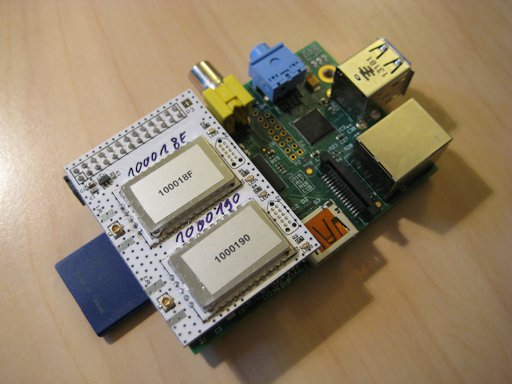
\includegraphics[width=\textwidth]{user_installation_guide/rpi.jpg}
		\caption{\gls{Raspberry Pi}}	
	\end{subfigure}
	\quad
	\begin{subfigure}[h]{\Imwidth\textwidth}
		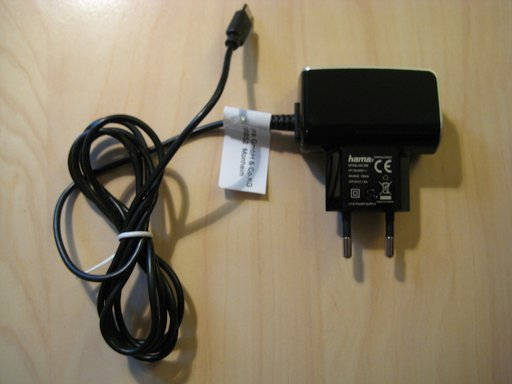
\includegraphics[width=\textwidth]{user_installation_guide/rpi-power-cord.jpg}
		\caption{\gls{Raspberry Pi} power cord}	
	\end{subfigure}
	\quad
	\begin{subfigure}[h]{\Imwidth\textwidth}
		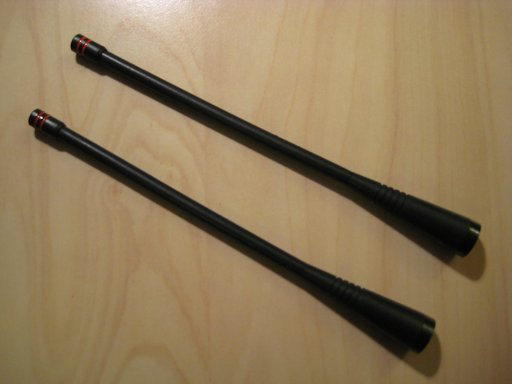
\includegraphics[width=\textwidth]{user_installation_guide/rpi-antenna.jpg}
		\caption{\gls{Raspberry Pi} antennas}	
	\end{subfigure}
	\quad
	\begin{subfigure}[h]{\Imwidth\textwidth}
		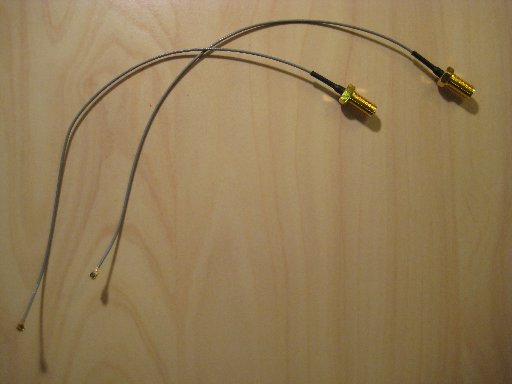
\includegraphics[width=\textwidth]{user_installation_guide/rpi-antenna-cable.jpg}
		\caption{Antenna signal cables}	
	\end{subfigure}
	\quad
	\begin{subfigure}[h]{\Imwidth\textwidth}
		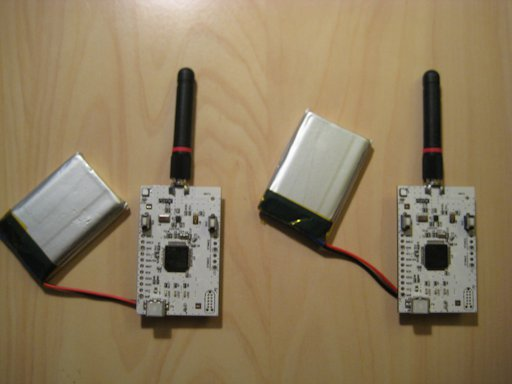
\includegraphics[width=\textwidth]{user_installation_guide/sensor.jpg}
		\caption{Sensors}	
	\end{subfigure}
	\quad
	\begin{subfigure}[h]{\Imwidth\textwidth}
		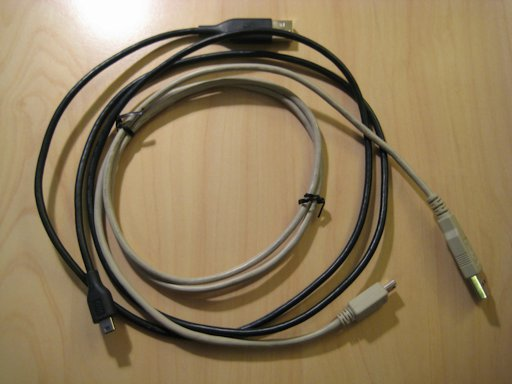
\includegraphics[width=\textwidth]{user_installation_guide/sensor-power-cord.jpg}
		\caption{Sensor power cords (optional)}	
	\end{subfigure}
	\quad
	\begin{subfigure}[h]{\Imwidth\textwidth}
		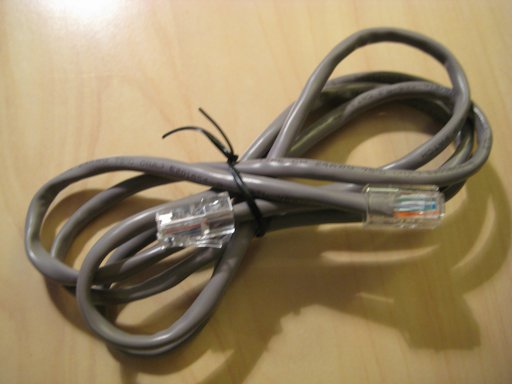
\includegraphics[width=\textwidth]{user_installation_guide/rpi-network-cable.jpg}
		\caption{Network cable}	
	\end{subfigure}
	\caption{Accessories needed to set up the central hub}
\end{figure}

To setup the central hub and the sensors, complete the steps outlined in the figures below:
\begin{figure}[H]
	\centering
	\begin{subfigure}[h]{0.48\textwidth}
		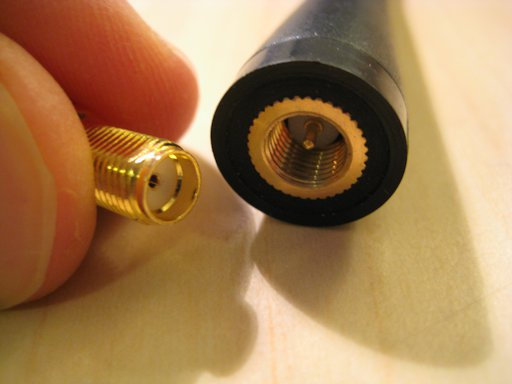
\includegraphics[width=\textwidth]{user_installation_guide/connect-antenna-cables.jpg}
	\end{subfigure}
	\quad
	\begin{subfigure}[h]{0.48\textwidth}
		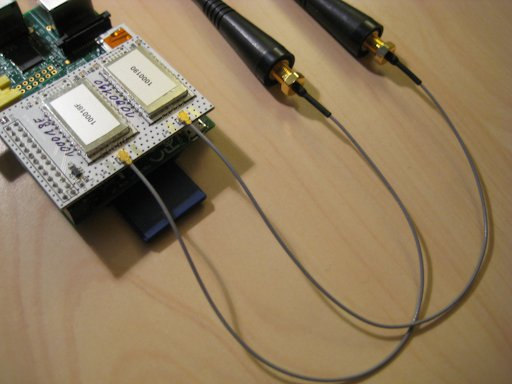
\includegraphics[width=\textwidth]{user_installation_guide/connect-rpi-antennas.jpg}
	\end{subfigure}
	\caption{Attach the antenna signal cables to the antennas, and connect the antenna signal cables to the \gls{Raspberry Pi}}
\end{figure}

\begin{figure}[H]
	\centering
	\begin{subfigure}[h]{0.48\textwidth}
		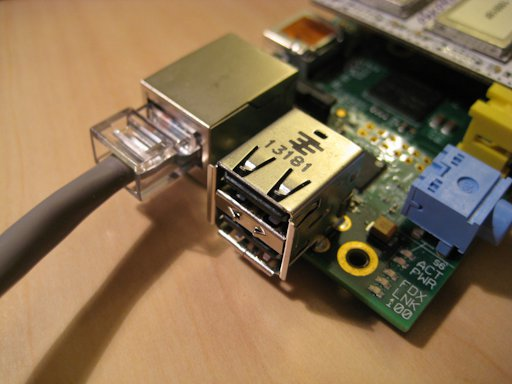
\includegraphics[width=\textwidth]{user_installation_guide/connect-rpi-network.jpg}
	\end{subfigure}
	\quad
	\begin{subfigure}[h]{0.48\textwidth}
		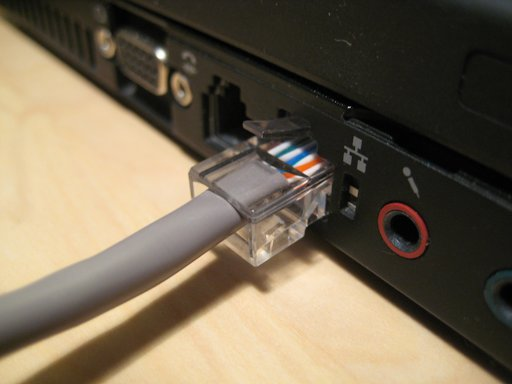
\includegraphics[width=\textwidth]{user_installation_guide/connect-rpi-network-2.jpg}
	\end{subfigure}
	\caption{Connect the \gls{Raspberry Pi} to the router using the networking cable}
\end{figure}

\begin{figure}[H]
	\centering
	\begin{subfigure}[h]{0.48\textwidth}
		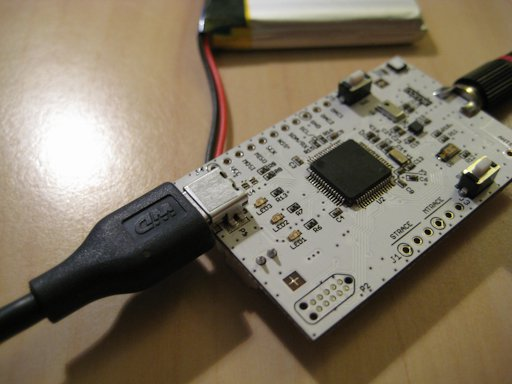
\includegraphics[width=\textwidth]{user_installation_guide/connect-sensor-power.jpg}
	\end{subfigure}
	\quad
	\begin{subfigure}[h]{0.48\textwidth}
		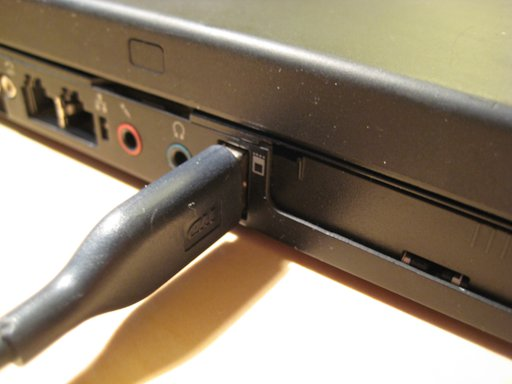
\includegraphics[width=\textwidth]{user_installation_guide/connect-sensor-power-2.jpg}
	\end{subfigure}
	\caption{Power the sensors by plugging one end of the sensor power cord into the sensor, and the other end into a powered USB port (optional).}
\end{figure}

\begin{figure}[H]
	\centering
	\begin{subfigure}[h]{0.48\textwidth}
		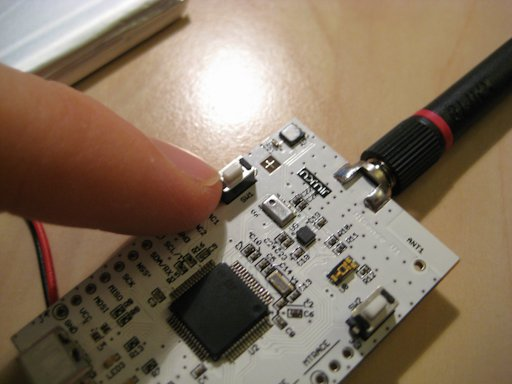
\includegraphics[width=\textwidth]{user_installation_guide/turn-on-sensors.jpg}
	\end{subfigure}
	\quad
	\begin{subfigure}[h]{0.48\textwidth}
		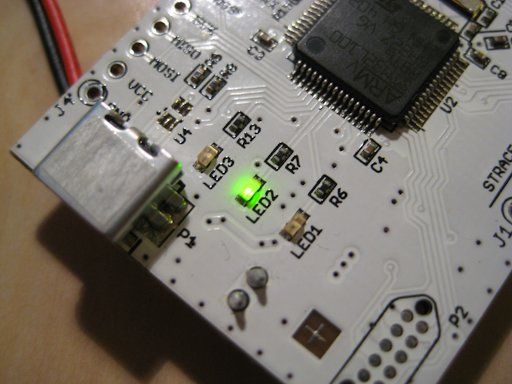
\includegraphics[width=\textwidth]{user_installation_guide/turn-on-sensors-2.jpg}
	\end{subfigure}
	\caption{Turn on the sensor by pressing the button to the left of the antenna. Keep the button depressed for at least one second, or until the green LED is lighted.}
\end{figure}

\begin{figure}[H]
	\centering
	\begin{subfigure}[h]{0.48\textwidth}
		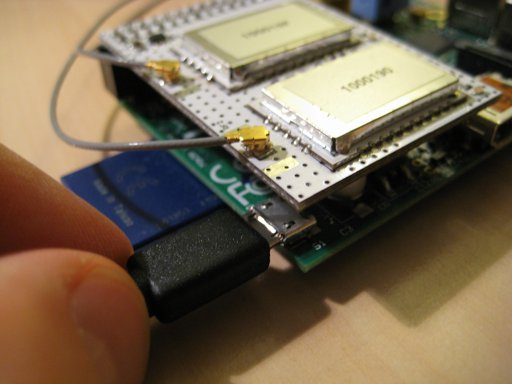
\includegraphics[width=\textwidth]{user_installation_guide/connect-rpi-power.jpg}
	\end{subfigure}
	\quad
	\begin{subfigure}[h]{0.48\textwidth}
		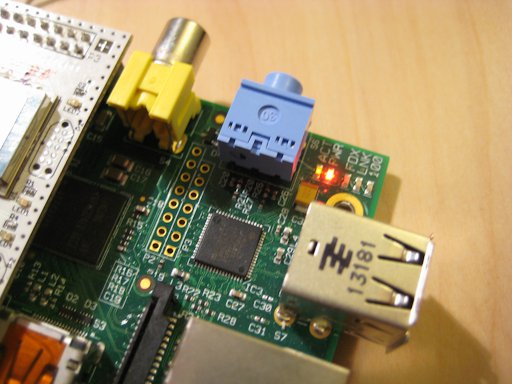
\includegraphics[width=\textwidth]{user_installation_guide/connect-rpi-power-2.jpg}
	\end{subfigure}
	\caption{Start the \gls{Raspberry Pi} by plugging the power cord into it. The other end of the cord should be plugged into a power outlet. A red LED will light up indicating that the Raspberry is powered.}
\end{figure}



\subsection{Acquiring IP Addresses}\label{subsec:acquiring_ip}
In order to set up all the components of the system, it is necessary to know the IP addresses of the central hub and the database. As these addresses are assigned dynamically by the \gls{DHCP} server, it is not possible to known them in advance. This section goes into detail about how to acquire the IP addresses.

For the central hub, the simplest way to discover the address is by trial and error. For this we need to know the address pool used by the \gls{DHCP} server, so take note of this when setting up the network. The idea is to test subsequent addresses from this pool until the address of the central hub is found. The central hub runs a \gls{REST}-based server, and the easiest way of testing an address is to type in the address in a browser. If the address is correct, this will open the configuration service of the central hub. It is likely that the central hub was leased an address in the lower end of the range, so it is a good idea to start there. For example, if the setup is performed on a local network, a typical lower end of the range address is 192.168.1.1.

If a laptop is used as a \gls{DHCP} server, another option is also available. This involves viewing the log messages written by the \gls{DHCP} server when the IP address was assigned. Likely, the \gls{DHCP} server will have written the addresses leases to the log, and it will be possible to acquire them.

It is also necessary to get the IP address of the database. Assuming the database is run on a computer with easy access to a terminal, this can be found using the command-line utility ipconfig in Windows, or ifconfig in OS X or Linux.

\paragraph{Using ipconfig in windows 7}
First it is necessary to open a Windows command prompt. This can be done from the windows start menu by typing "cmd" in the search field and pressing enter. To execute the ipconfig utility, type "ipconfig.exe" and press enter. This will print several network configuration parameters of the computer. The IP address of the database will be found at the end of the line containing the words "IP Address". An example output of the command is shown in the example below.

\lstset{style=custombash}
\begin{lstlisting}[caption=Example output of the ipconfig command in Windows]
Windows IP Configuration

Ethernet adapter Local Area Connection:

    Connection-specific DNS Suffix .  :
    Link-local IPv6 Address	   : fe80::9477:c944:e7dc:bb4f%14
    Autoconfiguration IP Address. . . : 172.16.0.24
    Subnet Mask . . . . . . . . . . . : 255.255.0.0
    Default Gateway . . . . . . . . . : 172.16.0.1
\end{lstlisting}


\paragraph{Using ifconfig in Linux}
In a terminal window, run the command "ifconfig" as show in the example below.

\lstset{style=custombash}
\begin{lstlisting}[caption=Example output of the ifconfig command in Linux]
$ ifconfig
wlan0  Link encap:Ethernet  HWaddr 00:18:de:01:f9:8c  
       inet addr:78.91.30.139  Bcast:78.91.31.255  Mask: ...
       inet6 addr: fe80::218:deff:fe01:f98c/64 Scope:Link
       UP BROADCAST RUNNING MULTICAST  MTU:1500  Metric:1
       RX packets:94186 errors:0 dropped:0 overruns:0 frame:0
       TX packets:90496 errors:0 dropped:0 overruns:0 carrier:0
       collisions:0 txqueuelen:1000 
       RX bytes:32612781 (31.1 MiB)  TX bytes:40241945 (38.3 MiB)
\end{lstlisting}



\subsection{Downloading the visualiser}\label{subsec:downloading_the_visualiser}
This section describes how to download the visualiser component as an executable jar file. The executable jar file can be downloaded by visiting the url
\url{https://github.com/audunx/tdt4290g10/raw/Prototype_C%2B%2B/visualiser-1.0-SNAPSHOT-jar-with-dependencies.jar}
\noindent in a browser, and save the file to a suitable location.



\subsection{Configuring the system}
Some of the different system components can be configured. These are the visualiser, and the central hub.

\subsubsection{Configuring the central hub}
The central hub and the sensors can be highly customized in how the central hub pulls data from the sensors. This configuration interface is accessed with a web browser, typing the IP address of the central hub into the address bar. Visiting the IP address should redirect the browser to a login screen. As before, use as login credentials ‘root’ as both username and password. A screenshot of the configuration interface is shown below.
\begin{figure}[H]\caption{Configuring the central hub using a browser}
	\centering
	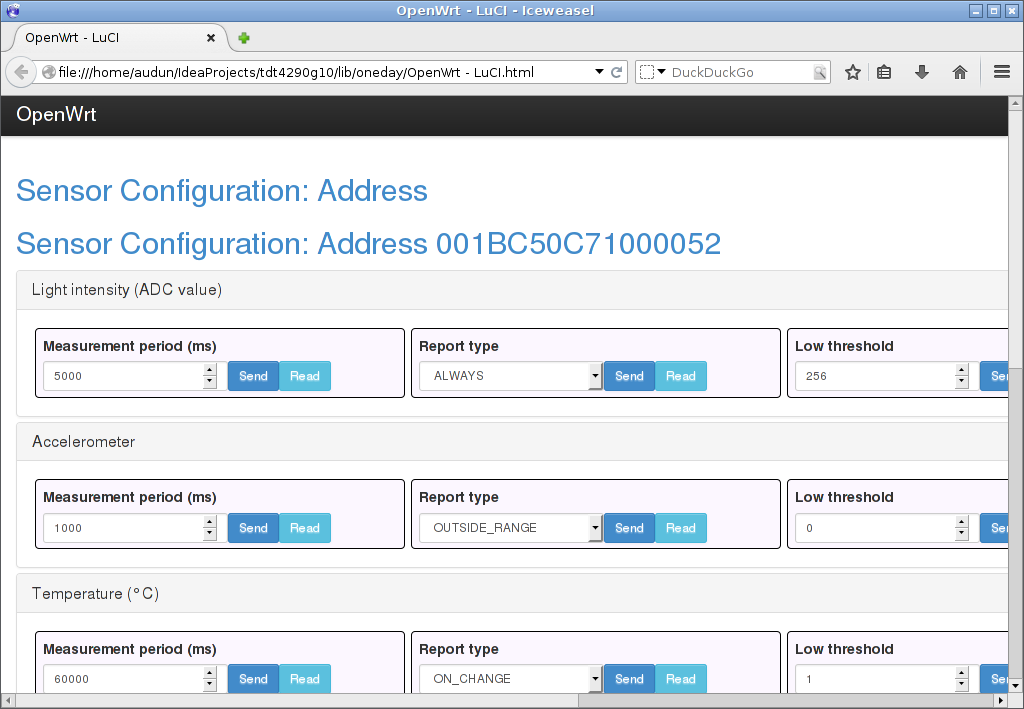
\includegraphics[width=\textwidth]{user_installation_guide/configure-central-hub.png}
\end{figure}

Using the configuration interface it is possible to configure the frequency with which sensors measure the different environment characteristics. It is also possible to configure several different kinds of thresholds for that specify how large a change should be before it is reported.

\subsubsection{Configuring the visualiser}
There are two aspects of the visualiser that can be configured. Notably, the unless the visualiser and the database are running on the same system, the visualiser needs to be configured with the IP address of the database. In addition, it is also possible to specify what the map view will use as maximum and minimum accepted values for the link budget. A link budget value exceeding a threshold will be set to the closest acceptable value. In order to configure the visualiser, a file named "visualiser.properties" should be created in the folder where the visualiser is run. This file may contain the link budget and database configuration elements as shown in the below example table:
\begin{table}[H]
	\centering
	\ttfamily
	\begin{tabular}{|ll|}\hline
		minLinkBudget &= 40		\\
		maxLinkBudget &= 100	\\
		databaseIpAddress &= 192.168.1.8	\\\hline
	\end{tabular}
\end{table}



\subsection{Starting the System Components}
At this point all devices are powered on, they are connected to the network, and the IP address of the central hub and the database has been acquired. The final step is to start the individual system components. These include the visualiser, the database, and a small script running on the \gls{Raspberry Pi}. The central hub is started automatically by the \gls{Raspberry Pi} on boot. It is important that the database already runs before the visualiser is started. Apart from that, the components can be started in any order. However, it is recommended to start them in the order specified below.

\subsubsection{Starting the Database}
The database receives sensor samples from the central hub, storing them in files. In order to start the database, open a terminal and navigate to the folder where the file the executable .jar file is located. Next, execute the .jar using the command
\lstset{style=custombash}[caption=Command to execute the database in Java.]
\begin{lstlisting}
$ java -jar IoT-service-0.9.1-SNAPSHOT-with-deps.jar
\end{lstlisting}
The database should now start printing log messages.



\subsubsection{Starting the pull script}
The script running on the \gls{Raspberry Pi} along with the central hub is used pull sensor samples from the central hub and push them to the database. It is a Bash script that uses the command-line tool cURL to communicate with the central hub and the database. This script resides on the central hub under the path \texttt{/home/root/push.sh}. The recommended way to start the script, is to log on to the \gls{Raspberry Pi} through ssh, using ‘root’ as both username and password. After logging in, the script is started with the command
\lstset{style=custombash}
\begin{lstlisting}
$ ./pull.sh <central hub ip> <database ip>
\end{lstlisting}
where the IP of the central hub and the database is specified as arguments. Optionally, the script can be run on any computer connected to the network. Using a Bash shell it can be pulled from the central hub with the command below.
\lstset{style=custombash}
\begin{lstlisting}
$ scp root@<central hub ip>:/home/root/pull.sh .
\end{lstlisting}
After copying, the script is executed with the same command used above when logging on to the \gls{Raspberry Pi}.

\subsubsection{Starting the Visualiser}
The visualiser is started by using java to execute the jar file downloaded in \subfullref{subsec:downloading_the_visualiser}. In most systems, double-clicking the file will execute it in java automatically.

Executing the visualiser by double-clicking it is probably the easiest way to run it. However, there is another method that gives more control over the program by making the program output visible. In order to read program output, the jar file needs to be executed in a console window. The rest of this section goes briefly through the details of this process for Windows and Linux systems.

\paragraph{Locating the visualiser jar using the Windows command prompt}
First open a command prompt as described in section \subfullref{subsec:acquiring_ip}. Then, use the command prompt to navigate to the folder where the jar file is located. The following command explains how you can navigate between folders using Windows command prompt:
\lstset{style=custombash}
\begin{lstlisting}[caption=Windows command to change current folder]
> cd "<file path>"
\end{lstlisting}
Putting the file path in quotes avoids issues with paths containing certain characters, such as spaces. Finding the full path of the file's location can be done by locating the file using Windows Explorer, and then copying the path from the address bar.

After navigating to the folder where the jar file is located, the jar file can be executed with a similar command to the one used to run the database:
\begin{lstlisting}[caption=Command to execute the visualiser in Java.]
$ java -jar visualiser-1.0-SNAPSHOT-jar-with-dependencies.jar
\end{lstlisting}



\subsection{Accessing the source code}
This section goes through some different methods for accessing the project source code in the group's public GitHub repository.

\subsubsection{Visiting GitHub.com in a browser}
The easiest way to browse the project source code is to use a browser to open the url: \url{https://github.com/audunx/tdt4290g10}. GitHub makes the repository accessible in an ordered fashion, and provides useful statistics as an aside.

\subsubsection{Cloning the repository with Git}
In order to work with the source code, the project should be cloned with Git using the clone url \texttt{https://github.com/audunx/tdt4290g10.git}. Git installation instructions for major operating systems can be found at \url{http://git-scm.com/book/en/v2/Getting-Started-Installing-Git}. Git documentation is found at the same site.



\end{document}
